\section{What can be learned when every exact target is hidden?}
Castelli et al.\ screened cubic perovskites for light-driven water splitting \cite{castelli}. A composition with a suitable gap can still fail on band alignment or stability. Problem D combines these failures into one score and asks for a single composition in each of two search spaces \cite{contest}. We can check predictions at thousands of public compositions, yet none attains zero loss. Q1 therefore evaluates a composition-only predictor on labeled pairs and scores the hidden set. Q2 and Q3 refit that predictor on all public labels and select a single material from a fixed-family and a three-family pool, respectively.

For ordered sites $A$ and $B$ and anion family $X$, denote formation energy, GLLB-SC gap, valence edge and conduction edge by $e,g,v,c$, respectively, in eV. GLLB-SC is a computational approach to estimating band gaps \cite{kuisma}. We retain the edge convention in the supplied data. The five penalties represent excessive formation energy, a gap below or above its window, and a violation of either band-edge threshold. With $[t]_+=\max(0,t)$ and all energy scales in eV, the dimensionless contest loss is
\begin{align}
 d&=(e-0.21,\;1.4-g,\;g-3.1,\;5.73-v,\;c-4.50),\notag\\
 V(A,B,X)&=\sum_{j=1}^5 [d_j/0.5]_+^2. \label{eq:loss}
\end{align}
Equation~\eqref{eq:loss} includes equality in its zero set. The organizers report 19 compositions with $V=0$ and 15 under the strict physical inequalities. We use the former convention. Recomputing $V$ from the four rounded public quantities gives a maximum absolute discrepancy of $1.02\times10^{-5}$. We fit the supplied six-decimal target after this check.

The partitions in Table~\ref{tab:data} keep all seven anion families of each ordered pair together.

\begin{table}[htbp]
\caption{Official partitions. Each pair contributes seven families to its partition. The hidden exact-target count comes from the organizers.}\label{tab:data}
\centering\begin{tabular}{lrrrr}
\toprule Partition & Pairs & Rows & $V=0$ & $V<1$ observed\\\midrule
Training (02) & 1,608 & 11,256 & 0 & 83\\
Selection (03) & 567 & 3,969 & 0 & 27\\
Holdout (04) & 529 & 3,703 & 19 & unavailable\\\bottomrule
\end{tabular}
\end{table}

The grid contains $52^2\times7$ compositions, including $A=B$. The pair sets are disjoint. The seven families are O3, NO2, FO2, N2O, N3, O2S and FNO. File 06 repeats public compositions without labels. We use 02 for Q1 training, 03 for model selection and 04 for predictions. Q2 and Q3 use a separate fit on 02 and 03. The problem permits pools 07 or 11 for Q2 and 08 or 12 for Q3. We solve the full pools and separately identify the best candidates among unseen pairs. Sorting by identifier breaks exact score ties. Inference excludes identifiers, measured geometry and outcomes of density functional theory (DFT) calculations.

\subsection{Why A and B must remain ordered}
In the ideal cubic perovskite setting, place A at the corners, B at the body center and the anions at the face centers \cite{aflow}. The eight corners contribute $8/8=1$ A atom per cell. The six faces contribute $6/2=3$ anions. B has six nearest anion neighbors in the illustrated octahedron, while the periodically repeated face centers give A twelve nearest anion neighbors. The contest family label specifies the composition of the three anions. For example, NO2 supplies one N and two O per formula unit. The files give no site-resolved O/N ordering for the blind candidate.

Figure~\ref{fig:cell} holds the ideal fractional coordinates fixed while exchanging the cations. Each panel's gap and violation come from its own public DFT record.

\begin{figure}[htbp]
\centering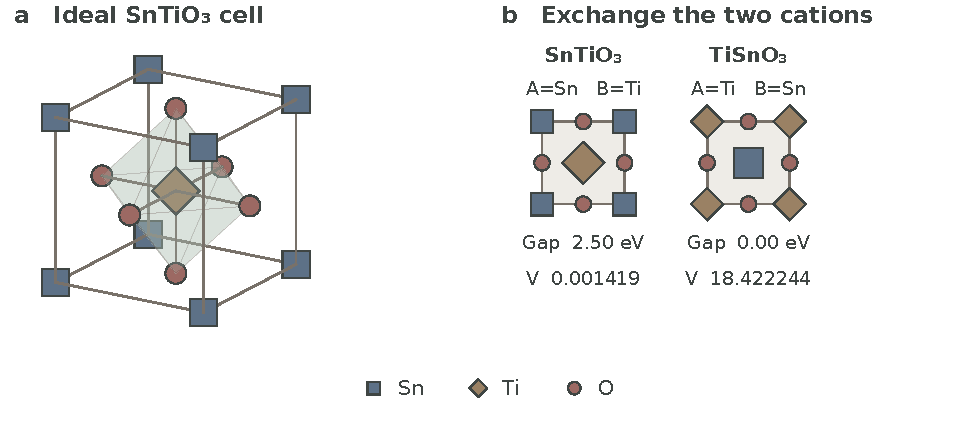
\includegraphics[width=.98\linewidth]{figures/crystal_sites.pdf}
\caption{Ordered sites in the ideal cubic prototype and two independently computed oxide records. In the unit cell Sn occupies the A corners and Ti the B center. The projected sections at right show the cations and equatorial oxygen sites. Squares mark Sn, diamonds Ti and circles O in both panels. Geometry follows the cubic prototype \cite{aflow}.}\label{fig:cell}
\end{figure}

We matched each public record $(a,b,x)$ with $(b,a,x)$ when both were labeled, excluded $a=b$, and counted each reciprocal pair once. Among 5,971 matches, the median absolute difference is 5.5296, with quartiles 2.2672 and 12.6046. A predictor that gives both records the same output $h$ incurs
\[
 \tfrac12\{|V(a,b,x)-h|+|V(b,a,x)-h|\}\ \geq\
 \tfrac12 |V(a,b,x)-V(b,a,x)|.
\]
Averaging the right-hand side gives an unavoidable MAE of at least 4.6805 on these 11,942 matched rows for a site-invariant predictor. This bound concerns the matched sample and must be compared on that same sample. It motivates retaining separate A and B descriptors before fitting.

The Sn--Ti pair illustrates the size of this effect. Public $\mathrm{SnTiO_3}$ has $g=2.50$ eV and $V=0.001419$. Its reversed assignment $\mathrm{TiSnO_3}$ has $g=0$ and $V=18.422244$. For $\mathrm{SnTiO_3}$ the supplied cubic lattice parameter is 3.969143~\AA. Lattice parameters and volumes are available only in labeled records and do not enter the score of a new composition.

\section{Problem 1. A lower bound for the metallic branch}
Of 15,225 public rows, 14,652 have $g=0$. On every one, $v=c$. Set both edges to $t$. The gap alone contributes $(1.4/0.5)^2=7.84$. Between 4.50 and 5.73, the two edge penalties form a convex quadratic symmetric about $t=5.115$. Outside that interval their sum increases. Formation energy can only add a nonnegative penalty. Hence under the observed coincident-edge convention
\begin{equation}
 V_{\rm metal}\ \geq\ L=7.84+
 \frac{(5.73-4.50)^2}{2(0.5)^2}=10.8658. \label{eq:metal}
\end{equation}
The smallest metallic values observed against the bound in Eq.~\eqref{eq:metal} are 10.865834 in training and 10.866614 in validation. A zero-gap record thus teaches the model where a near-target is physically unlikely. At prediction time the gap is unknown.

\subhead{Reading the lower bound in the public records}
The metallic lower bound resolves the gap and both edge penalties jointly. For a metal with common edge $t$, the vertical distance above the curve below equals the formation-energy penalty up to rounding.
\[
 B(t)=7.84+[ (5.73-t)/0.5 ]_+^2+[(t-4.50)/0.5]_+^2 .
\]
Moving the common edge to the left alleviates the CBM violation while increasing the VBM violation. Moving it to the right has the opposite effect. Their thresholds are separated by 1.23 eV. Figure~\ref{fig:regimes} shows why neither edge adjustment can compensate for zero gap.

\begin{figure}[htbp]
\centering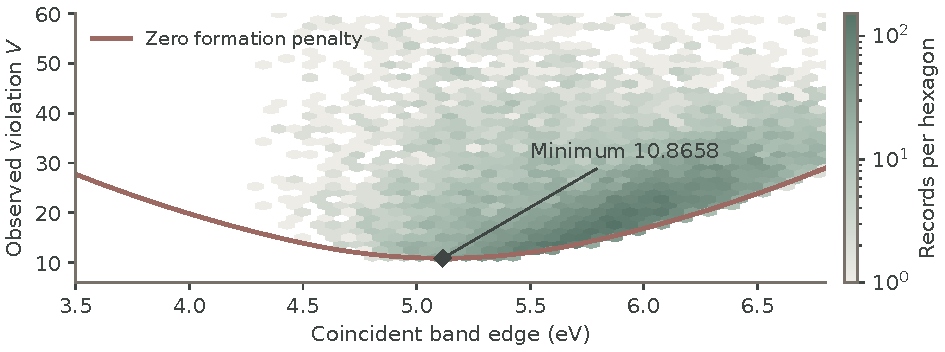
\includegraphics[width=\linewidth]{figures/physical_regimes.pdf}
\caption{Zero-gap records in files 02 and 03, grouped into hexagons in the displayed window. The color scale counts records. The curve gives the lower bound $B(t)$ and the diamond marks its minimum at $t=5.115$ eV.}\label{fig:regimes}
\end{figure}

Positive gap narrows the public screen from 15,225 records to 573 and retains all 110 with $V<1$. Even with the true gap known, only $110/573=19.2\%$ of the gapped records pass this relaxed test. In O3, 28 of 132 gapped compositions have $V<1$. In NO2, the ratio is 14 of 70, and in N3 none of 18 passes. These counts are descriptive. In particular, the hidden set was constructed to contain the exact targets, which changes the interpretation of any full-population prevalence estimate.


\subhead{A surrogate with observable training labels}
Composition-based descriptors have proved useful in inorganic property prediction \cite{ward}. For each metal site separately we use atomic number, Pauling electronegativity, periodic-table row and group from pymatgen \cite{ong}. Three categorical fields $A,B,X$ bring the total to eleven. This preserves site order and assumes the supplied cubic prototype throughout.

CatBoost handles the categorical inputs \cite{catboost}. Let $p(z)$ estimate $\Pr(g>0\mid z)$ from composition features $z$. Two regressors estimate $V$ conditional on positive and zero gap. The law of total expectation motivates
\begin{equation}
 \Vh(z)=p(z)\max(0,f_+(z)) + (1-p(z))\max(L,f_0(z)).
 \label{eq:mix}
\end{equation}
File 02 supplies 432 positive-gap and 10,824 metallic outcomes for fitting the gate. This classification label is observed even though the exact screening target never occurs in 02. Soft weighting keeps every candidate eligible. A composition receiving a high $p$ may still fail the band-edge or formation-energy requirements.

We compare with one direct regressor for $V$ using identical descriptors, 350 boosting iterations per component, depth 5, learning rate 0.08, four CPU threads and seeds 26 and 42. The mixture fits three components. Holding depth and descriptors fixed, we also fit direct regressors with 700 and 1,050 trees. The first budget matches the nominal training-row passes of the gate plus its two disjoint branches, and the second matches their total tree count. We carry seed 26 forward to use one fixed score table for both optimization problems. File 03 was reused for exploratory model selection. Its metrics describe development performance. The Q1 deliverable, \texttt{q1\_holdout.csv}, contains one composition-only prediction for each of the 3,703 hidden IDs.

\subsection{Following one composition through the predictor}
Consider $\mathrm{InTiO_3}$, the first-ranked seed-26 mixture candidate in the Q3 validation subset. Its actual zero gap is available only when we evaluate the prediction. During screening, the classifier puts probability 0.5426 on a positive gap. The two regressors then disagree by 9.3786 score units. Figure~\ref{fig:gate} traces the two weighted contributions in Eq.~\eqref{eq:mix} and compares their sum with the public DFT-derived loss.

\begin{figure}[htbp]
\centering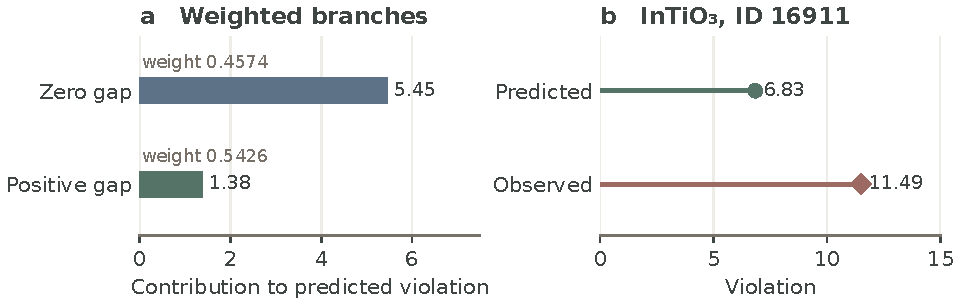
\includegraphics[width=\linewidth]{figures/gate_mechanism.pdf}
\caption{The composition-only gate for validation ID 16911 assigns positive-gap probability 0.5426. The bars give the contributions after weighting. The public loss was used only for evaluation.}\label{fig:gate}
\end{figure}

Writing $m$ and $u$ for the clipped metallic and positive-gap scores, respectively, gives $\Vh=m-p(m-u)$. The metallic branch contributes approximately $0.4574(11.9231)=5.45$ and the positive-gap branch $0.5426(2.5444)=1.38$. The arithmetic explains two features of this selection. First, a hard decision at $p=0.5$ would report only 2.5444, discarding a material portion of the expected violation. Second, a 0.10 increase in the positive-gap probability would lower the score by 0.938 with both branch estimates fixed. That sensitivity is large enough to matter among closely ranked candidates.

The gate also imposes a one-sided condition on very low scores. Since $u\geq0$ and $m\geq L$, Eq.~\eqref{eq:mix} gives
\[
 \Vh\geq (1-p)L,\qquad
 \Vh<1\ \Longrightarrow\ p>1-1/L\simeq0.9080 .
\]
This is a necessary condition on a \emph{predicted} score below one. A physically good but uncertain material may still receive a much larger score. Ranking by the continuous mixture keeps that material available when no candidate crosses a fixed prediction threshold. Conversely, assigning probability greater than 0.908 does not guarantee good band alignment or formation energy.

\subsection{A controlled test of the probability gate}
To isolate the effect of gating, we hold the learned branch functions $u$ and $m$, the seed, descriptors and train--validation split fixed. Only the mixing weight changes across the comparisons in Table~\ref{tab:gate}. The constant rule assigns the file-02 positive-gap fraction $432/11256$ to every composition. The hard rule replaces the predicted probability by $\mathbf{1}[p\geq0.5]$. The soft rule uses $p$ itself. A fourth, diagnostic rule routes each validation record by its observed gap label, an input unavailable on the blind pool. Replaying the soft rule reproduces all 3,969 archived validation scores within $10^{-8}$.

\begin{table}[htbp]
\caption{Changing only the gate on file 03. Hits count $V<1$ among the first 50. All-family and Q3 denominators are 27 and 11 available near-targets. The final column gives observed $V$ at Q3 rank one.}\label{tab:gate}
\centering\small\begin{tabular}{lrrrr}
\toprule Routing weight & All-family MAE & All hits & Q3 hits & Q3 first $V$\\\midrule
Training prevalence & 2.942 & 4 & 2 & 10.895\\
Hard decision & 2.909 & 8 & 1 & 11.492\\
Soft probability & 2.949 & 13 & 5 & 11.492\\
Observed gap (diagnostic) & 2.678 & 20 & 9 & 1.488\\\bottomrule
\end{tabular}
\end{table}

The hard decision gives a slightly smaller mean error than the soft mixture, yet it retrieves five fewer near-targets at budget 50 across all families. Many promising compositions fall below the hard threshold. Of the 141 validation materials with a positive gap, the classifier flags only 14 at $p\geq0.5$, alongside four false positives. Its precision there is $14/18$, while its recall is $14/141$. A hard rule makes the 127 missed positive-gap records share the metallic scoring regime with most of the validation set.

As a probability score for the positive-gap event, the gate attains a Brier score of 0.0273, compared with 0.0343 for the constant training prevalence. Average precision is 0.367 against a validation event frequency of 0.0355. These metrics assess the positive-gap event. No exact contest target occurs in the public labels. On Q3, even access to the observed regime yields a first choice with $V=1.4884$, above the near-target threshold. Improving the gate alone would still leave the regression problem of ranking positive-gap materials by their joint physical penalties.

\section{Validation at the actual screening budget}
For an ordered shortlist $S_k$ define $H_k=\sum_{i\in S_k}\mathbf1[V_i<1]$. Recall divides $H_k$ by the number of such targets in the relevant pool. For a one-choice decision $i^*$, labeled-pool regret is $R_1=V_{i^*}-\min_i V_i$. The expected number of $V<1$ hits in 50 random draws without replacement from the entire validation pool is $50(27/3969)=0.34$. Table~\ref{tab:val} compares this screening budget with the first-choice outcomes.

\begin{table}[htbp]
\caption{Performance on 567 unseen ordered pairs. Mean absolute error (MAE), root mean squared error (RMSE) and hits use all 3,969 rows. The last columns give observed $V$ at rank one in each restricted pool.}\label{tab:val}
\centering\small\begin{tabular}{lrrrrrrr}
\toprule Fit & Seed & MAE & RMSE & $H_{20}$ & $H_{50}$ & Q2 first & Q3 first\\\midrule
Direct &26&3.016&5.000&2&6&8.562&11.492\\
Mixture &26&2.949&4.828&8&13&10.927&11.492\\
Direct &42&3.013&4.945&3&10&11.540&46.240\\
Mixture &42&3.025&4.902&9&15&11.084&12.670\\\bottomrule
\end{tabular}
\end{table}

The mixture retrieves 48.1\% and 55.6\% of the 27 near-targets at $k=50$ for seeds 26 and 42. In Q2 it retrieves all four validation near-targets in 50 checks under both seeds, yet its first choice has $V>10$. In Q3, the seed-26 mixture and direct fits retrieve five and one of eleven near-targets. Both select $\mathrm{InTiO_3}$ first, with regret $11.49225-0.04000=11.45225$ (Figure~\ref{fig:screen}). Increasing the direct-model tree count to 700 and 1,050 raises its Q3 hit count from one to two and four at seed 26, with the same first choice. At seed 42 the counts are three, five and five, against six for the mixture. The shortlist advantage narrows as the direct model grows. The supplementary curves show both seeds and all pools (Figure~\ref{fig:allbudgets}).

\begin{figure}[htbp]
\centering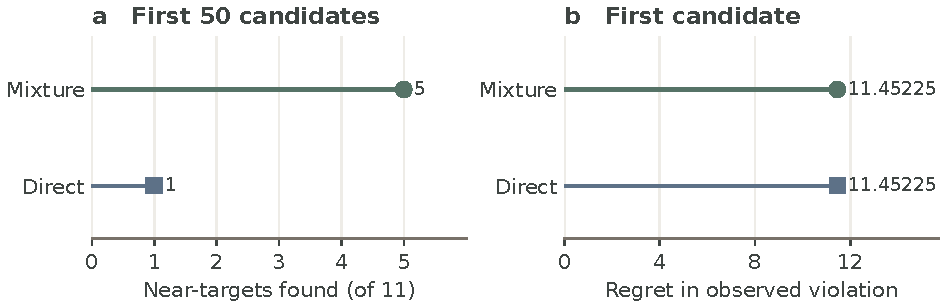
\includegraphics[width=.97\linewidth]{figures/q3_budget.pdf}
\caption{Screening at two budgets on the same 1,701 Q3 validation compositions, seed 26. Left, hits among the first 50, with a near-target defined by $V<1$. Right, the excess observed violation of the first choice over the attainable minimum.}\label{fig:screen}
\end{figure}

\subsection{How much of the shortlist survives a change of sample or seed?}
The validation sample contains 567 ordered metal pairs. Each pair contributes seven associated families, and we use the pair as the resampling unit. To assess sensitivity to the mix of pairs, we draw 567 pairs with replacement, retaining the whole family group and its multiplicity. On each resample we rank the records using the already fitted seed-26 predictors and count $V<1$ hits among the first 50. Figure~\ref{fig:stability} uses the same draw for both methods. This paired design preserves the dependence of their predictions on the same materials.

\begin{figure}[htbp]
\centering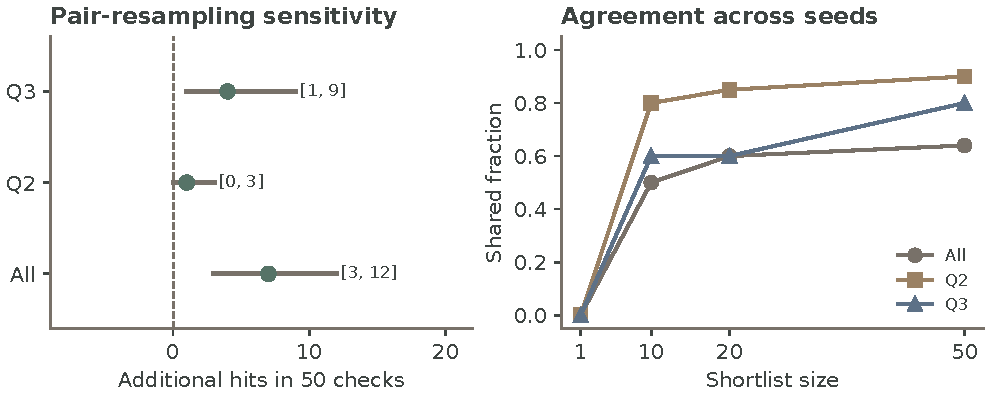
\includegraphics[width=\linewidth]{figures/validation_stability.pdf}
\caption{Left, observed mixture-minus-direct hit counts at budget 50 (dots) and the 2.5th to 97.5th percentiles over 2,000 resampled pair sets (segments). Right, the fraction of each mixture shortlist shared by training seeds 26 and 42 on the original validation set.}\label{fig:stability}
\end{figure}

Across all families the observed improvement is seven hits, with a resampling range of three to twelve. For Q2 the improvement is one and the interval reaches zero. Only four near-targets are present in that validation pool, leaving little room for a large observed gain. For Q3 the gain is four with a range of one to nine. The intervals describe sensitivity conditional on the trained models and the empirical pair distribution. Resampled duplicates count toward both hit totals and the 50-record budget. These are diagnostics of the metric, rather than prospective yields for 50 distinct new experiments.

We separately intersect the predicted shortlists from seeds 26 and 42. At $k=50$, 45 of 50 Q2 candidates and 40 of 50 Q3 candidates are shared. At $k=1$ the two seeds select different IDs in both pools. We therefore report the first choice on the frozen score table together with its validation regret. Seed agreement at a larger budget supports a follow-up shortlist but supplies little assurance about which single material a laboratory should measure first.

\section{Unseen pairs, withheld near-targets and a failed alternative}
We repeat the comparison inside file 02 with five shuffled folds of complete $(A,B)$ pairs. Each model uses four folds for fitting and ranks the fifth. Spending 50 checks in each held-out pool gives 250 checks per row of Table~\ref{tab:fold}. The five regrets describe variability across held-out compositions. The folds overlap in training data.
\begin{table}[htbp]
\caption{Five grouped folds within 02. The denominator counts all observed $V<1$ targets across the five held-out pools.}\label{tab:fold}
\centering\small\begin{tabular}{llrrr}
\toprule Pool & Method & Hits / targets & Median $R_1$ & Range of $R_1$\\\midrule
\FoldRows
\bottomrule\end{tabular}
\end{table}
In Q3 the mixture finds more near-targets over the five shortlists, yet its median first-choice regret is larger. A second stress test removes every pair containing $V<0.25$ from the training portion of file 02 and adds background pairs to form a 322-pair holdout. All 29 such targets lie among 2,254 held-out records. Across two background selections, direct regression retrieves five of 29 in its top 50 and the mixture retrieves nine. On the three-family subset the counts are five and seven of 20. Mixture rank-one $V$ moves from 13.8461 to 0.4756 while the attainable minimum is 0.0004 in both. These runs share the same targets. Their prevalence is 1.29\%, compared with 0.10\% for exact zeros on the contest grid.

\subhead{When predicting each physical quantity helps}
A public note suggested predicting the four physical properties first \cite{note1}. A second note discusses retaining metallic records for classification and regression \cite{note2}. Four separate 220-tree regressions predict $e,g,v,c$, followed by Eq.~\eqref{eq:loss}. At seeds 26 and 42, the property model selects a Q2 composition with observed $V=0.36$, versus 10.93 and 11.54 for a 220-tree direct fit. In Q3 both property fits choose $\mathrm{CaZrO_3}$ with $V=46.24$. At seed 26 its predicted gap is 2.19 eV, inside the window. The observed gap is 6.50 eV. The upper-gap term alone is $((6.50-3.10)/0.50)^2=46.24$. Average property accuracy conceals this error at the selected extreme. We carry the mixture forward for a common score table across both pools and its stronger shortlist performance. For a single Q2 choice, the property-first result favors that alternative on the available validation set.

\subsection{Reading a near miss and a false positive from their band edges}
The band-edge thresholds and gap window test different properties. Figure~\ref{fig:bands} compares the contest's two reported edges with their cutoffs and places the modeled and public gaps for $\mathrm{CaZrO_3}$ on a separate axis.

\begin{figure}[htbp]
\centering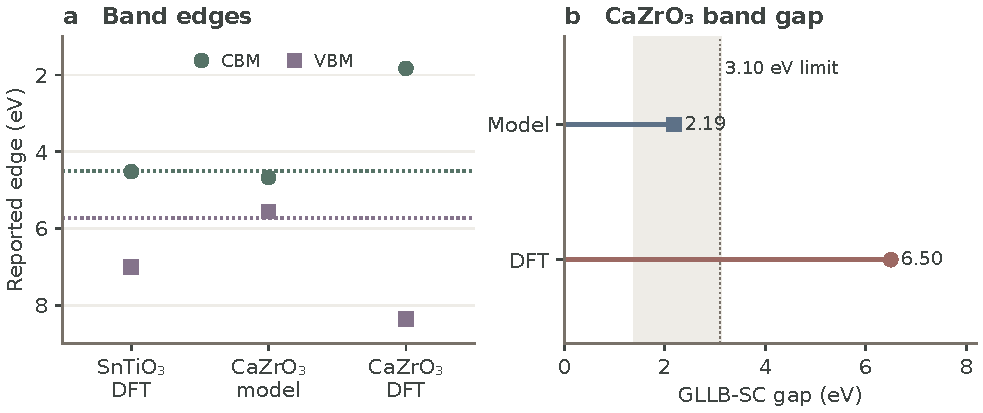
\includegraphics[width=\linewidth]{figures/band_edges.pdf}
\caption{Public DFT values and seed-26 property-model estimates. Left, the dotted lines mark the CBM (4.50 eV) and VBM (5.73 eV) cutoffs on the contest's inverted edge axis. Right, shading marks the 1.40--3.10 eV accepted gap interval.}\label{fig:bands}
\end{figure}

For $\mathrm{SnTiO_3}$, the CBM lies 0.018833 eV beyond its cutoff, a difference too small to resolve easily at the figure scale. For $\mathrm{CaZrO_3}$ the observed edges both pass, but the observed gap is 6.50 eV. It exceeds the upper limit by 3.40 eV and produces the entire observed violation of 46.24.

The modeled band edges help explain how the four-property model can rank that material first. It predicts $g=2.1883$ eV, with both small band-edge violations and a passing formation energy, for a total predicted $V=0.2342$. Its independently fitted edges imply $5.5559-4.6680=0.8879$ eV, far from its own gap estimate. In the public DFT record the analogous difference is 6.53 eV, close to the tabulated 6.50 eV. The discrepancy between the model's two estimates of the gap provides a composition-level warning that could be checked before spending a single assay. The following sensitivity test evaluates this warning across all Q3 validation pairs.

\subsection{Can a consistency check rescue a one-choice screen?}
The $\mathrm{CaZrO_3}$ failure suggests a testable diagnostic. Define
\[
 D(z)=\big|\hat g(z)-(\hat v(z)-\hat c(z))\big|.
\]
All three terms are predictions from the property-first model, so the diagnostic could be computed before measuring a candidate. It checks whether the two representations of the gap agree. A small residual can also occur when both representations are wrong in the same direction.

We test a veto on the 1,701 Q3 validation records. We discard predictions with $D>\tau$ and select the remaining candidate with the smallest property-first violation. Table~\ref{tab:veto} reports both seeds, with 26 first in each entry. The same 11 near-targets are available to each fit. Thresholds are exploratory, and this test does not alter the frozen mixture.
\begin{table}[htbp]
\caption{Cost of vetoing inconsistent property predictions. Entries give seed 26 / seed 42. Counts refer to distinct Q3 validation records.}\label{tab:veto}
\centering\small\begin{tabular}{lrrr}
\toprule Tolerance (eV) & Eligible records & Near-targets retained & First observed $V$\\\midrule
No veto & 1701 / 1701 & 11 / 11 & 46.24 / 46.24\\
1.00 & 1698 / 1699 & 11 / 10 & 11.25 / 46.24\\
0.50 & 1690 / 1681 & 10 / 9 & 11.97 / 11.25\\
0.25 & 1634 / 1623 & 7 / 5 & 11.97 / 10.88\\
0.05 & 753 / 805 & 0 / 3 & 10.88 / 10.93\\\bottomrule
\end{tabular}
\end{table}

At $\tau=0.50$ the large error on $\mathrm{CaZrO_3}$ is removed for both seeds, yet neither replacement is a near-target. At $\tau=0.05$ the seed-26 screen eliminates every available near-target. Agreement between model outputs can flag a case for inspection. Using that agreement as an automatic rejection criterion sacrifices some of the materials the screen is meant to find.


